\documentclass[twocolumn]{aastex61}
%\documentclass[preprint]{aastex}
%\documentclass[aps,prd,preprint,showpacs,superscriptaddress,amsmath]{revtex4}
%\documentclass[prd,showpacs,superscriptaddress,twocolumn,
%floatfix,preprintnumbers,altaffilletter]{revtex4}
%\documentclass[prd,showpacs,superscriptaddress,
%floatfix,preprintnumbers,altaffilletter]{revtex4}

\usepackage{longtable}
\usepackage{graphicx}
\usepackage{amsmath,amssymb}
\usepackage{color}
\usepackage{units}
\usepackage{epstopdf}
\usepackage{hyperref}
\usepackage{multirow}
\usepackage{float}
\usepackage{tikz}
%\usepackage{subcaption}
%\captionsetup{compatibility=false}
\usetikzlibrary{shapes,arrows}

\usepackage{listings}
\usepackage{color}

\definecolor{dkgreen}{rgb}{0,0.6,0}
\definecolor{gray}{rgb}{0.5,0.5,0.5}
\definecolor{mauve}{rgb}{0.58,0,0.82}

\lstset{frame=tb,
  language=python,
  aboveskip=3mm,
  belowskip=3mm,
  showstringspaces=false,
  columns=flexible,
  basicstyle={\small\ttfamily},
  numbers=none,
  numberstyle=\tiny\color{gray},
  keywordstyle=\color{blue},
  commentstyle=\color{dkgreen},
  stringstyle=\color{mauve},
  breaklines=true,
  breakatwhitespace=true,
  tabsize=3
}

%\usepackage[doublespacing]{setspace}

\newcommand{\braket}[2]{\left\langle#1\, |\,#2\,\right\rangle}  %  < #1 | #2 >
\newcommand{\expec}[1]{\langle#1\rangle}  %  < #1 >
\newcommand{\drm}{{\rm d}}
\newcommand{\irm}{{\rm i}}
\newcommand{\beq}{\begin{equation}}
\newcommand{\eeq}{\end{equation}}
\newcommand{\bdm}{\begin{displaymath}}
\newcommand{\edm}{\end{displaymath}}
\newcommand{\T}[1]{\tilde{#1}}
\newcommand{\wT}[1]{\widetilde{#1}}
\newcommand{\Cdot}{\!\cdot\!}
\newcommand{\SNR}{\textnormal{SNR}}
\newcommand{\rednote}[1]{{\color{red} (#1)}}
\definecolor{Gray}{gray}{0.9}
\definecolor{orange}{rgb}{0.9,0.5,0}
\newcommand{\td}[1]{{\textcolor{orange}{\texttt{TD: #1}} }}

\graphicspath{{./plots/}}
\begin{document}

\title{gwemopt: Optimizing searches for electromagnetic counterparts of gravitational wave triggers}

\author{Man Leong Chan}
\affil{University of Glasgow, Glasgow G12 8QQ, United Kingdom}

\author{Deep Chatterjee}
\affil{University of Wisconsin-Milwaukee, Milwaukee, WI 53201, USA}

\author{Michael Coughlin}
\affil{Department of Physics, Harvard University, Cambridge, MA 02138, USA}

\author{Shaon Ghosh}
\affil{University of Wisconsin-Milwaukee, Milwaukee, WI 53201, USA}

\author{Giuseppe Greco}
\affil{INFN, Sezione di Firenze, I-50019 Sesto Fiorentino, Firenze, Italy}

\author{Yiming Hu}
\affil{TianQin Research Center for Gravitational Physics, Sun Yat-sen University, Tangjiawan, Zhuhai 519082, Guangdong, P. R. China}

\author{Shasvath Kapadia}
\affil{University of Wisconsin-Milwaukee, Milwaukee, WI 53201, USA}

\author{Javed Rana}
\affil{Inter-University Centre for Astronomy and Astrophysics, Pune 411007, India}

\author{Om Sharan Salafia}
\affil{INAF - Osservatorio Astronomico di Brera Merate, via E. Bianchi 46, I–23807 Merate, Italy}

\author{Duo Tao}
\affil{Carleton College, Northfield, MN 55057, USA}

\begin{abstract}

Documentation for gwemopt

\end{abstract}

%\maketitle

\section{Introduction}
\label{sec:Intro}

There has been significant effort expended in the search for the electromagnetic counterpart of the gravitational waves found by compact binary black hole systems \citep{AbEA2016a,AbEA2016g,AbEA2017}.
In general, there is significant optimism for the potential counterparts for emission from binary neutron star and black hole - neutron star systems across timescales and wavelengths \citep{Nakar2007,MeBe2012}. 
The scientific output from a joint gravitational-wave and electromagnetic observation is expected to be significant. For example, detection of a kilonova coincident with a gravitational wave would allow for the exploration of r-process nucleosynthesis in the unbound ejecta from a merger involving a neutron star \cite{MeBa2015}.
In addition, a joint observation with a short gamma-ray burst would not only confirm that these phenomena are driven by compact binary mergers, but also allow for the study of their beaming, energetics, and galactic environment \cite{MeBe2012}.

To facilitate the detection of gravitational-wave counterparts, probability skymaps as a function of sky direction and distance are released for gravitational wave triggers produced by the detectors \citep{SiPr2014,BeMa2015}. 
Due to the significant sky coverage required to observe the gravitational-wave sky localization regions, usually spanning $\approx 100\,\textrm{deg}^2$, techniques to optimize the followup efforts are of significant utility \citep{Fair2009,Fair2011,Grover:2013,WeCh2010,SiAy2014,SiPr2014,BeMa2015,EsVi2015,CoLi2015,KlVe2016}.
Given the large sky localization regions involved, wide-field survey telescopes have the best opportunities to make a detection. 
The Panoramic Survey Telescope and Rapid Response System (Pan-STARRS) \citep{MoKa2012}, Asteroid Terrestrial-impact Last Alert System (ATLAS) \citep{Ton2011}, the intermediate Palomar Transient Factory (PTF) \citep{RaSh2009} and (what will become) the Zwicky Transient Facility (ZTF), BlackGEM \citep{BlGr2015} and the Large Synoptic Survey Telescope (LSST) \citep{Ivezic2014} are all examples of such systems.
For example, Pan-STARRS has a 7$^\circ$ field of view (FOV), achieving a 5 $\sigma$ limit of 21.5 (AB mag) in the i band in a 45 second exposure. ATLAS has a 29.2$^\circ$ field of view, achieving a 5 $\sigma$ limit of 18.7 in the cyan band in a 30 second exposure. For comparison, LSST will have a $9.6\textrm{deg}^2$ FOV and will require a 21\,s r-band exposure length to reach 22 mag.

Due to the significant difference in telescope configurations, including FOV, filter, typical exposure times, and limiting magnitudes, in addition to placement on the earth and therefore different seeing and sky conditions, optimizing gravitational wave followups for generic telescopes is difficult. Therefore, in the following, we will take the telescopes mentioned above as examples. 

For this reason, we have created a codebase named \emph{gwemopt} that utilizes methods from a variety of recent papers geared towards optimizing efforts of followup. We employ methods to read gravitational-wave skymaps and the associated information made available from GraceDB \footnote{https://gracedb.ligo.org}, in addition to information about the telescopes to tile the sky, allocate available telescope time to the chosen fields, and schedule that time in a way that optimizes based on expected lightcurves.
In section~\ref{sec:algorithm}, we describe the algorithm.
In section~\ref{sec:performance}, we describe the performance of the algorithms.
In section~\ref{sec:conclusions}, we offer concluding remarks and suggest directions for future research.

\section{Algorithm}
\label{sec:algorithm}

Figure~\ref{fig:flowchart} shows the flowchart for the \emph{gwemopt} pipeline, developed to optimize the efforts of electromagnetic followup of gravitational-wave events. \emph{gwemopt} is developed in python, which has the benefit of interfaces to both LIGO's gravitational-wave candidate event database (GraceDB) and HEALPIX \citep{GoHi2005}, the format in which LIGO reports skymaps.

It uses events provided by gracedb in addition to information about the telescopes to creating tiles and optimize time allocations in the fields.
It uses information about potential lightcurves from electromagnetic counterparts to schedule the available telescope time.
In the following, we will describe the calculations that go into creating tiling, time allocations, and observing sequences from the skymaps.
We will account for both diurnal and observational constraints and have the possibility of imaging over many nights.

% Define block styles
\tikzstyle{decision} = [diamond, draw, fill=blue!20,
    text width=4.5em, text badly centered, node distance=3cm, inner sep=0pt]
\tikzstyle{block} = [rectangle, draw, fill=blue!20,
    text width=5em, text centered, rounded corners, minimum height=3em]
\tikzstyle{line} = [draw, -latex']
\tikzstyle{cloud} = [draw, ellipse,fill=red!20, node distance=3cm,
    minimum height=2em]
\tikzstyle{emptyblock} = [rectangle, minimum height=3em]

\begin{figure}[t]
 \begin{center}
 \begin{tikzpicture}[node distance = 2.3cm, auto]
    % Place nodes
    \node [emptyblock] (init) {};
    \node [block, left of=init] (GraceDB) {GraceDB};
    \node [block, right of=init] (Telescope) {Telescope};
    \node [block, below of=init] (Tiling) {Tiling of the field of view};
    \node [block, below of=Tiling] (Time) {Calculate time allocations};
    \node [block, below of=Time] (Schedule) {Schedule observations};
    \node [block, below of=Schedule] (Efficiency) {Calculate efficiencies};
    % Draw edges
    \path [line] (GraceDB) -- (Tiling);
    \path [line] (Telescope) -- (Tiling);
    \path [line] (Tiling) -- (Time);
    \path [line] (Time) -- (Schedule);
    \path [line] (Schedule) -- (Efficiency);
 \end{tikzpicture}
 \end{center}
 \caption{A flow chart of the \emph{gwemopt} pipeline.}
 \label{fig:flowchart}
\end{figure}

\subsection{GraceDB}

\begin{figure}[t]
\hspace*{-0.5cm}
\centering
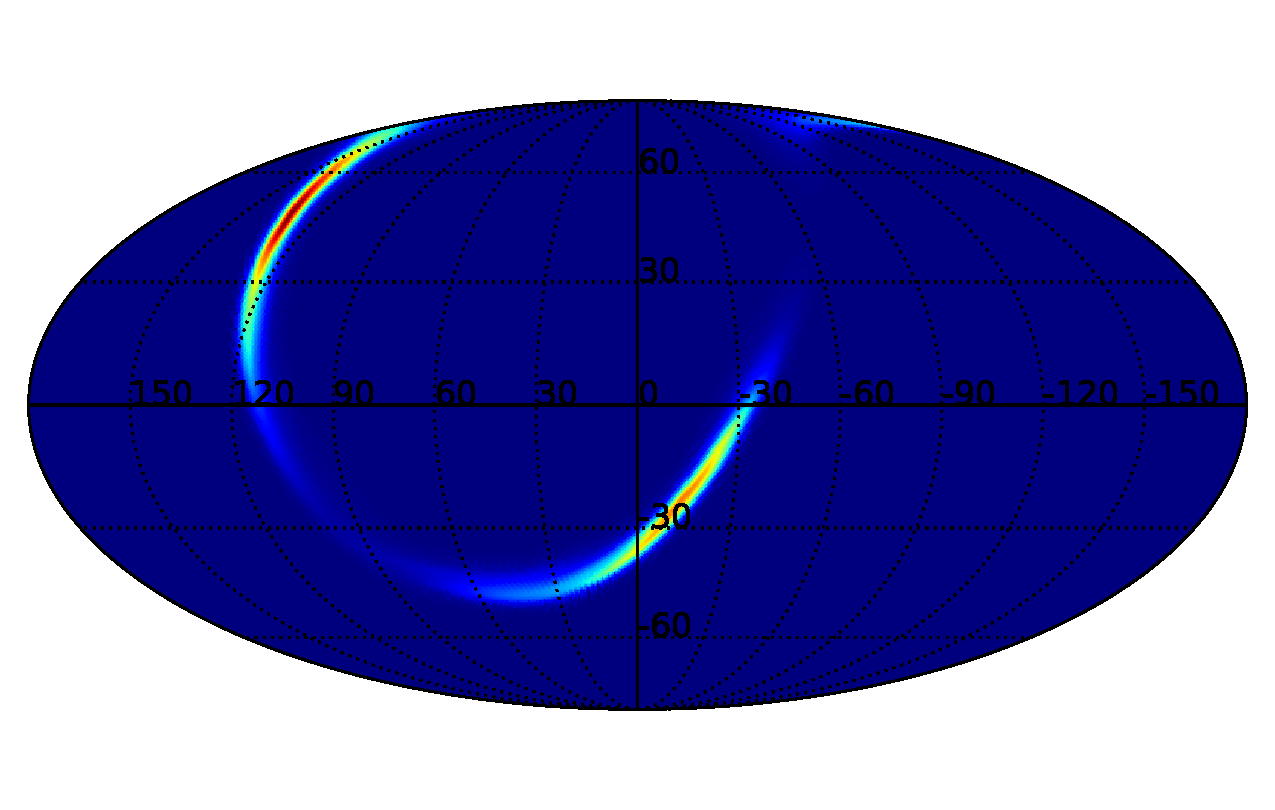
\includegraphics[width=3in]{prob.pdf}
\caption{The gravitational-wave likelihood $L_\textrm{GW}(\alpha,\delta,R)$ for GW170104.}
 \label{fig:skymap}
 \end{figure}

\begin{lstlisting}
python gwemopt_run --doEvent --do3D --event G268556
\end{lstlisting}

GraceDB is a service that provides information on candidate gravitational-wave events and the multi-messenger followups performed on them. An API is made available that allows for access to this information.
\emph{gwemopt} uses this API to access information pertinent for gravitational-wave followups.
First of all, it downloads the gravitational-wave skymap for a given event; an example is shown in figure~\ref{fig:skymap}.
In addition, information such as the time of the event, the time delay between the time-of-arrival at the detectors, and \rednote{EM bright} information is noted.
\subsection{Telescope configuration}
\begin{lstlisting}
python gwemopt_run --doEvent --do3D --telescope LSST
\end{lstlisting}
\begin{table*}[t]
\scriptsize
\centering
\begin{tabular}{|c|c|c|c|c|c|c|c|c|}
\hline
Telescope & Latitude {[}deg{]} & Longitude {[}deg{]} & Elevation {[}m{]} & FOV {[}deg{]} & FOV shape & Filter & Exp. time {[}s{]} & Lim. Mag. \\ \hline
ATLAS          & 20.7204            & -156.1552           & 3055.0            & 5.46                                      & Square              & c      & 30.0                  & 18.7               \\ \hline
Pan-STARRS     & 20.7204            & -156.1552           & 3055.0            & 2.8                                       & Circle              & i      & 45.0                  & 21.5               \\ \hline
BlackGEM       & -29.2612           & -70.7313            & 2400.0            & 2.85                                      & Square              & g      & 300.0                 & 23.0               \\ \hline
LSST           & -30.1716           & -70.8009            & 2207.0            & 1.75                                      & Circle              & r      & 30.0                  & 24.4               \\ \hline
ZTF            & 33.3563            & -116.8648           & 1742.0            & 6.86                                      & Square              & r      & 30.0                  & 20.4               \\ \hline
\end{tabular}
\caption{Configuration of telescopes.}
\label{table:config}
\end{table*}
We require standardized configuration files for the telescopes to be analyzed. 
The information includes the filter being used, the limiting magnitude of the instrument and the exposure time required to achieve that magnitude, site location information, and information about the field of view shape and size. For the field of view, two options, square and circle are available, with the FOV being specified by the length of the square side and the radius of the circle. In addition, a tesselationFile is requested. This is especially useful for telescopes such as ZTF which use fixed telescope pointings which ensures the availability of reference images. In case a tesselation file is not available, one is automatically generated, described in the next section.
Configuration files for ATLAS, BlackGEM, LSST, PS1, and ZTF are available.
Table~\ref{table:config} provides the information assumed for these telescopes.\\
\subsection{Skymap tiling}
\begin{lstlisting}
python gwemopt_run --doEvent --do3D --doTiles --doPlots --tilesType ranked
\end{lstlisting}
There are a variety of algorithms in the literature for sky-map tiling, and the ones implemented in \emph{gwemopt} will be detailed below. The idea is to cover the sky with tiles the size of the telescope's field-of-view with minimal overlap. In some cases, these tiles are pre-determined by survey constraints in order to simplify difference imaging. In other cases, it is possible to optimize the tile locations based on the gravitational-wave skymaps, such that the tiles maximize the probability contained. In the following, we will check the difference between these tile locations to determine their effect. Due to the fields-of-view for these telescopes being in general much smaller than the probability region, the effect is expected to be relatively minimal.

\begin{figure*}
    \centering
    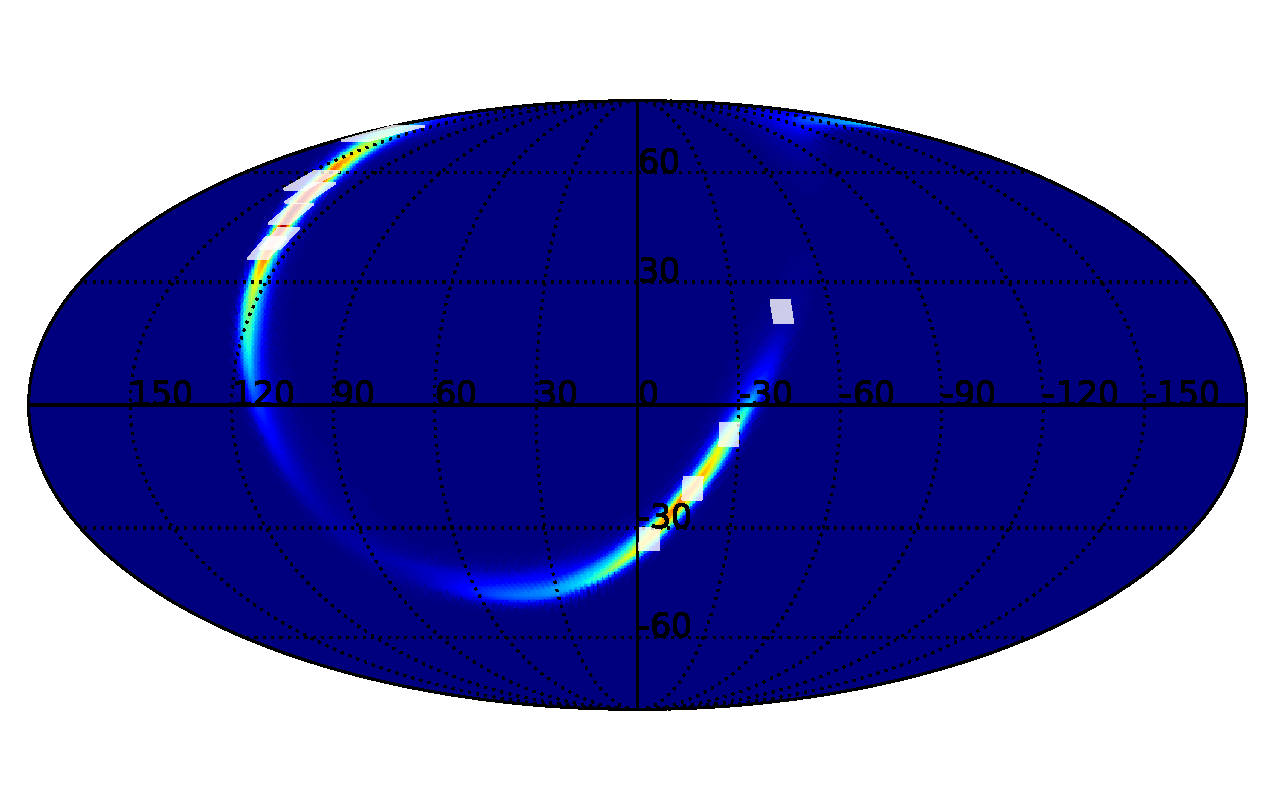
\includegraphics[width=3in]{tiling_greedy}
    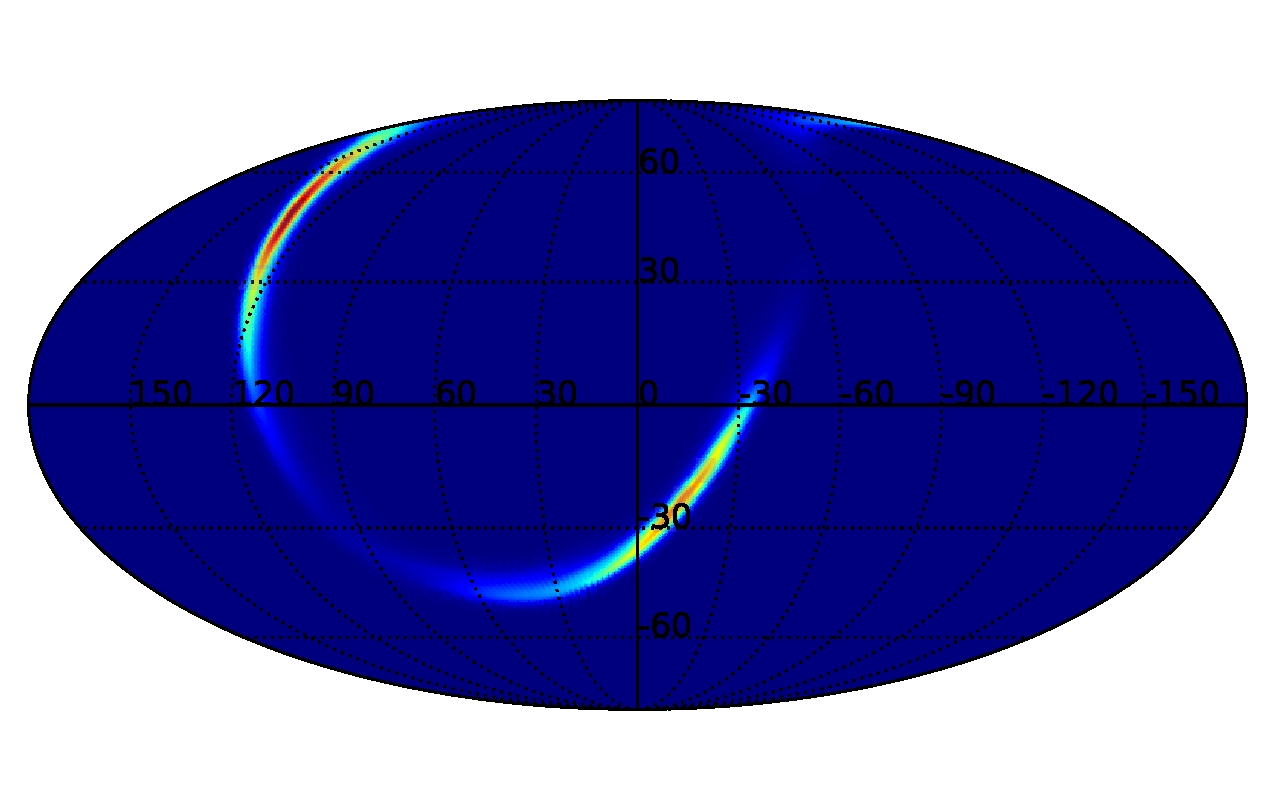
\includegraphics[width=3in]{tiling_hierarchical}
    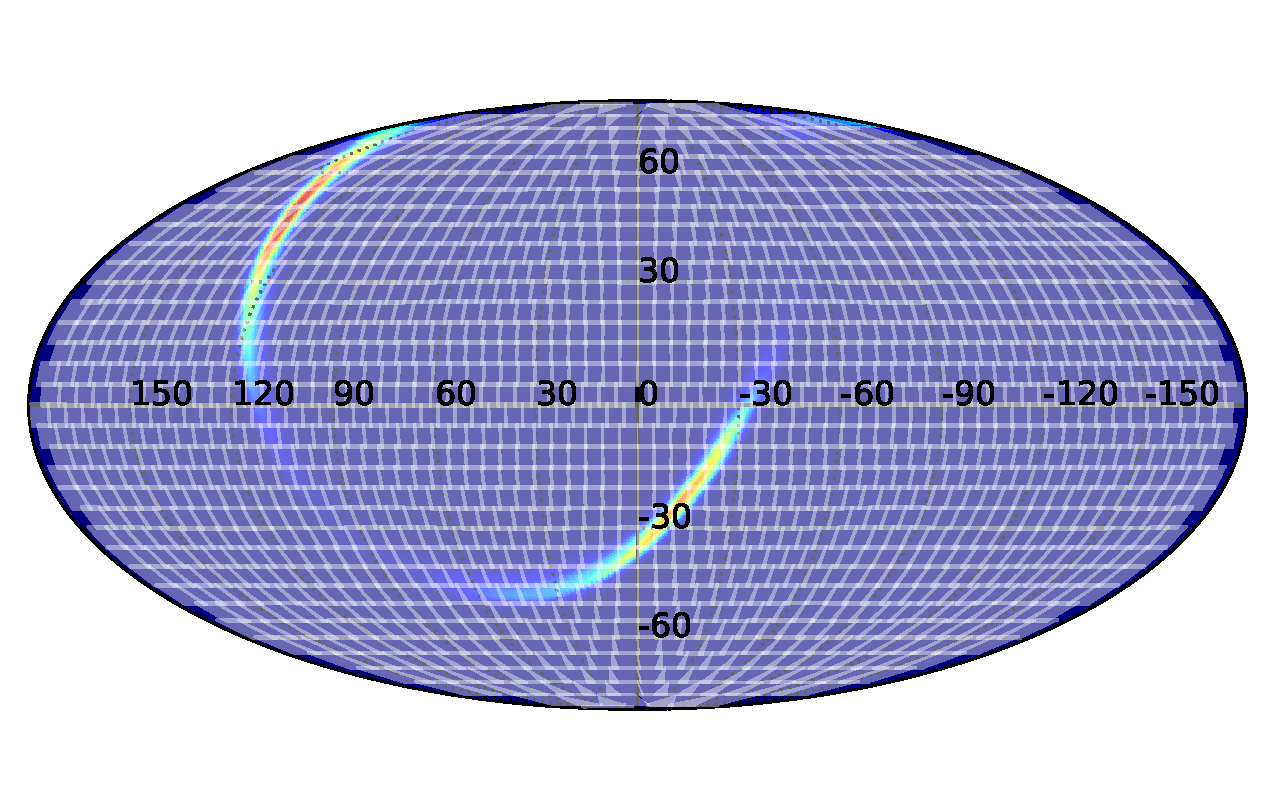
\includegraphics[width=3in]{tiling_moc}
    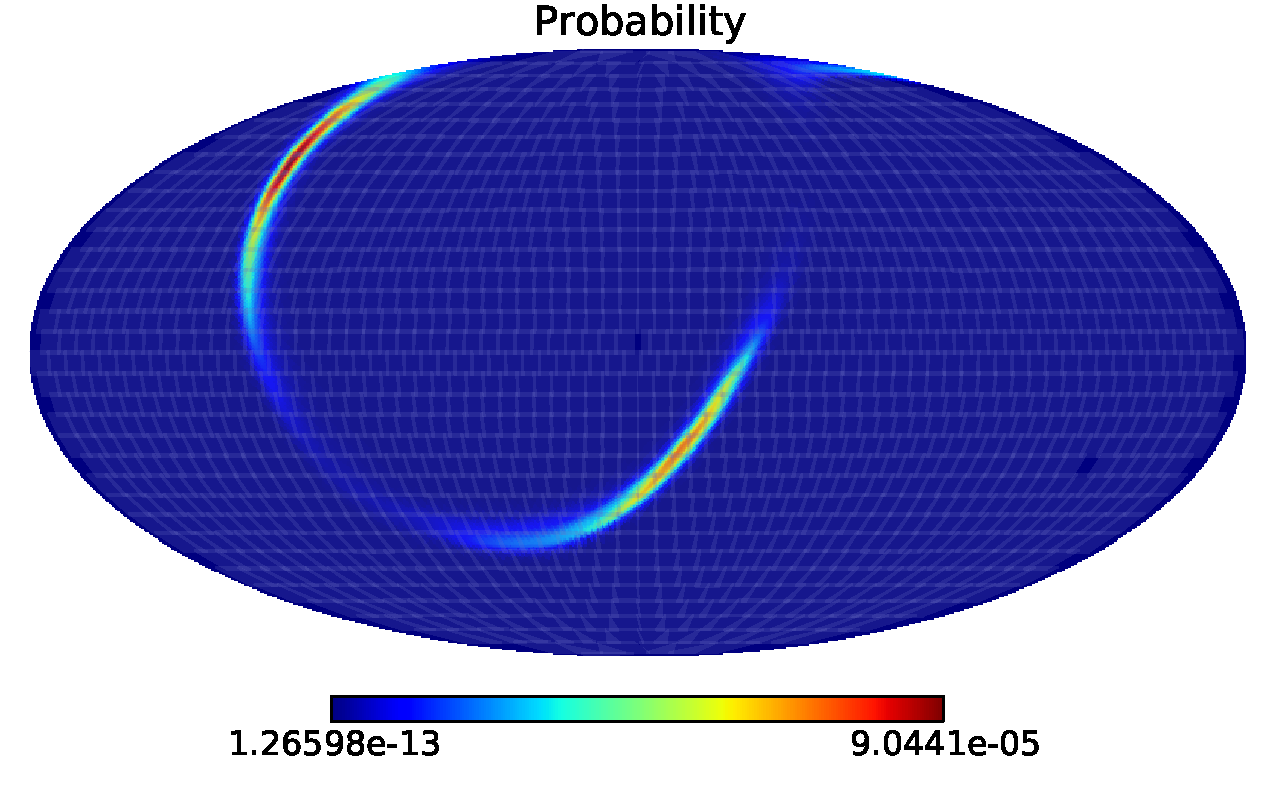
\includegraphics[width=3in]{tiling_ranked}
    \caption{Example outputs of different tiling algorithms. On the top left is the greedy version with Ntiles = 10, on the top right is the hierarchical version with the same, on the bottom left is the MOC skymap, and on the bottom right is the ranked skymap tiling.}
    \label{fig:tiling}
\end{figure*}

Gravitational-wave skymaps in general contain metrics that report the spatial probability of a gravitational-wave source lying within a certain location.
They are composed of HEALPIX arrays that encode either the 2D probability, in right ascension and declination, or 3D probability, which includes fits to the distance uncertainties.
They are reported in particular number of pixels, usually $\textrm{N}_\textrm{side} = 512$. 
This can introduce quantization errors, especially for small field-of-view telescopes. 
The --nside flag allows for the over- or under-sampling of the skymaps in the analysis.
This can introduce quantization errors of \rednote{XXX} \% for the field-of-view we consider here.

There are four options related to skymap tiling currently available, moc, ranked, hierarchical and greedy.

\rednote{Duo: all of these descriptions could use some expansion, especially the hierarchical and greedy schemes.}

\emph{moc}. Multi-order coverage of healpix maps hierarchically predefines cells in order to specify arbitrary sky regions \citep{FeBo2014}. MOC is proposed in order to provide fast set operations between regions on the sky. In MOC, the spherical sky is recursively divided into 4 regions and each region is a diamond. The process is demonstrated in Fig.\ref{fig:tiling_moc_demo}, where we can see that the sphere is divided recursively into four diamonds. The division stops according to the resolution necessary for a particular usage.

Here are two relevant implementation details about MOC.
\begin{itemize}
\item MOC uses equatorial coordinate system. 
\item MOC numbers each tile as such: the initial tile is numbered 0 on level 0. Then if we divided it, we get tile 0, 1, 2, 3 on level 1. if we start from a tile numbered M, its children will be numbered $M\times 4$, $M\times 4 + 1$, $M\times 4 + 2$,$M\times 4 + 3$ on the next level.
\end{itemize}
\begin{figure}[t]
\hspace*{-0.5cm}
\centering
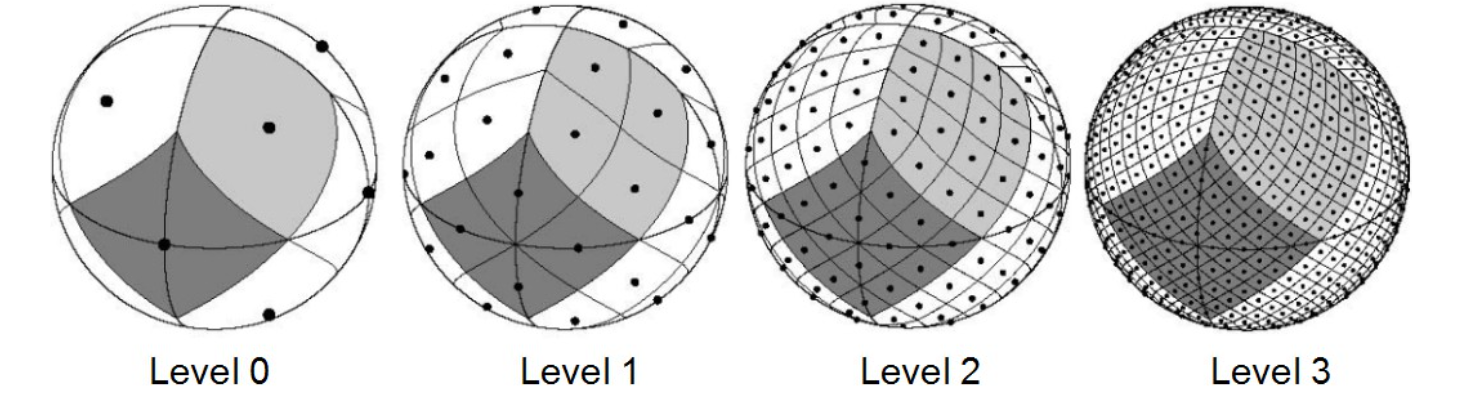
\includegraphics[width=3in]{tiling_moc_demo.png}
\caption{Diagram of the MOC tiling algorithm. The sky is divided into four diamond regions in level 0, 16 regions in level 1, 64 regions in level 2 and so on.}
 \label{fig:tiling_moc_demo}
 \end{figure}

\emph{ranked}. \cite{GhBl2016} use pre-defined sky cells. This tiling scheme is also based on a grid system with grids of equal sizes such as the one used by MOC. The sizes of the grids are the same as the size of the telescope FOV. For each tile in the grid at $(\alpha_i, \delta_i)$, we calculate a double integral that accumulates the probability distribution in this tile, shown in Eq.\ref{eqn:tile_ranked}.
\begin{equation}\label{eqn:tile_ranked}
T_{ij} = \int_{\alpha_i}^{\alpha_i+\Delta \alpha}\int_{\delta_i}^{\delta_i+\Delta \delta}L(\alpha, \delta)d\Omega
\end{equation}
Then we rank all the tiles with their $T_{ij}$ and select from the top of the rankings until we reach the target probability of 95\%.

\emph{hierarchical}. A Multinest based optimization which optimizes tiles for a given skymap by placing them sequentially. This method starts by selecting the tile that covers the most probability. Then, it sets the probability in that tile to be zero before going to the next iteration, when it again selects the tile that covers the most probability. It stops until a user-specified number of tiles are selected. The tiles selected might overlap on the corners when there are higher probability distributions around that corner. 
 
\emph{greedy}. An emcee based optimization which optimizes tiles for a given skymap by placing them simultaneously. This method selects tiles that cover the highest probability altogether from the skymap. It ranks all possible tiles and select from the top. Thus, the tiles selected by greedy method might overlap a lot when the probability distribution is concentrated.

\subsection{Time allocations}
\begin{lstlisting}
python gwemopt_run --doEvent --doPlots --doTiles --doSchedule --timeallocationType coverage
\end{lstlisting}
Once the tile locations have been assigned, whether dynamically or having been fixed previously, the next task is to assign time allocations to each tile, based on a variety of metrics. 
Because telescopes have fields of view that are in general significantly smaller than the probability region and typical exposure times for these telescopes are of order minutes (see Table~\ref{table:config}), it is not possible to image the entire probability region to interesting limiting magnitudes in a reasonable amount of time.
There are further constraints that arise from the diurnal cycle, observing time available for followup, limitations on the pointing a particular telescope is capable of, and the rise and set of tiles.
The following algorithms use a variety of methods to optimize the probability of imaging a counterpart.

The amount of time allocated is defined by a few constraints. 
First of all, segments are generated based on the observing time allocated after the gravitational-wave event. In the analyses that follow, the default will be to assume the next 3 days are available.
The segments are then intersected with night time at the site of the particular telescope.
This defines the segments available for the analysis.
The time available for the analysis is then determined from these segments.
This assumes implicitly that the electromagnetic counterpart has not faded beyond detection limits in the time available. Some of the time allocation algorithms below will use models to determine when the counterpart is expected to be too faint to be detectable.

There are four options related to time allocations as a function of sky location available, powerlaw, WAW, PEM, and coverage. Figure~\ref{fig:timealloc} shows examples of the powerlaw, WAW, and PEM types.

\rednote{Duo: In addition to expanding these descriptions based on your reading, I think it makes sense to try to state in a common mathematical formalism what each tries to do.}

\emph{Coverage.} This is an option whereby coverage from existing surveys, including the right ascension and declination of the pointing and the limiting magnitude, are used.

\emph{Powerlaw.} Many searches have used a variation on simply scaling the time allocation proportional to the probability skymaps, a technique employed in the Powerlaw method below. \cite{CoSt2016a} derived scaling relations for the time allocated to any given field, $t_i$, given the graviational-wave likelihood. We showed that under certain assumptions, $t_i \propto \left(\frac{L_\textrm{GW}(\alpha_i,\delta_i)}{a(\alpha_i,\delta_i)}\right)^{2/3}$, where $L_\textrm{GW}(\alpha_i,\delta_i)$ is the gravitational-wave likelihood and $a(\alpha_i,\delta_i)$ is Galactic extinction.  While the powerlaw based analysis is straightforward, it does not account for the fact that the telescope must be sensitive enough to detect the counterpart. In this sense, this algorithm is the least model dependent. Although the detectability is model-dependent, both in the distances returned by the gravitational-wave detectors and the absolute magnitude of the sources, the following algorithms account for this in multiple ways.

\emph{WAW (Where and when).} \cite{SoCo2017} use counterpart lightcurve models in the optical, infrared and radio constructed from information from the gravitational-wave signals to create a time- and sky location dependent probability for detecting electromagnetic transients.

\emph{PEM (Probability of electomagnetic counterpart).} \cite{ChHu2017} optimize the number of fields to observe and their time allocations by adopting priors on the intrinsic luminosity of the sources and using knowledge of distance to the counterparts provided for compact binary coalescence.

\begin{figure*}
    \centering
    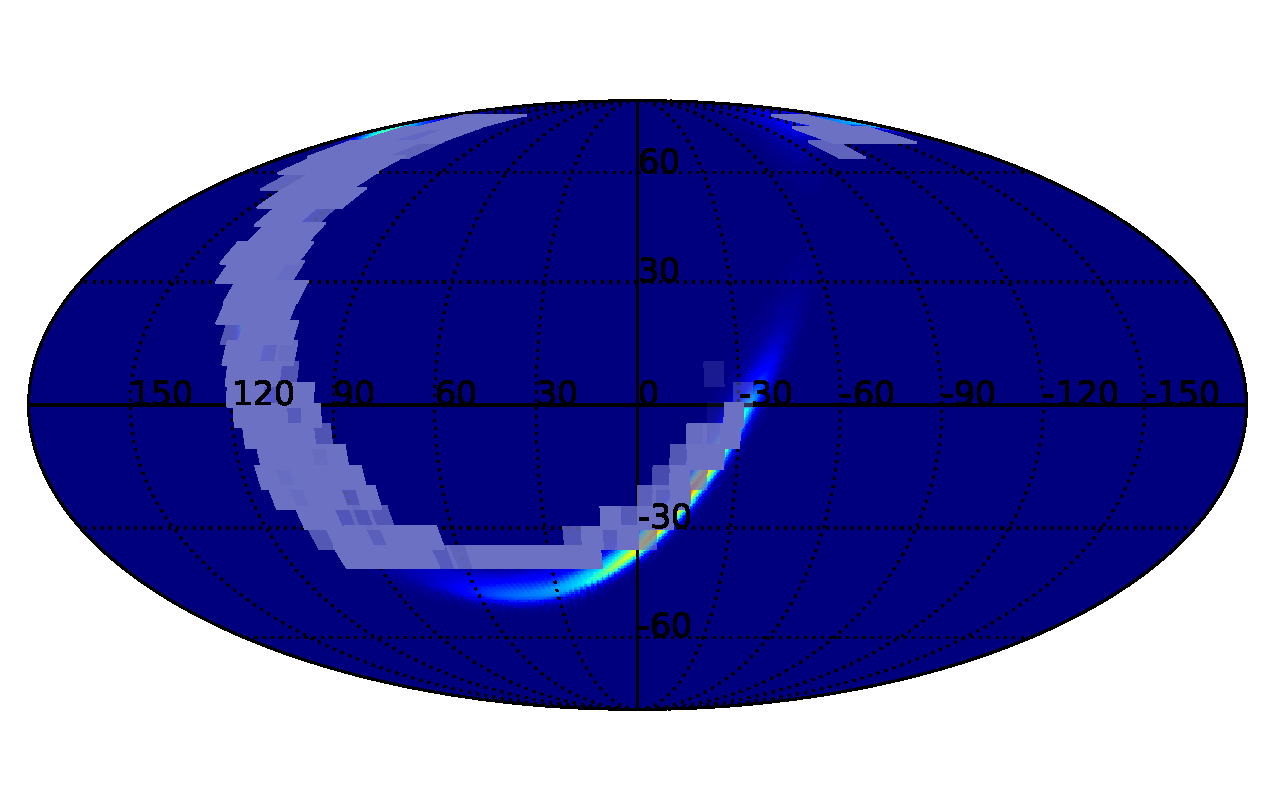
\includegraphics[width=3in]{timealloc_pem}
    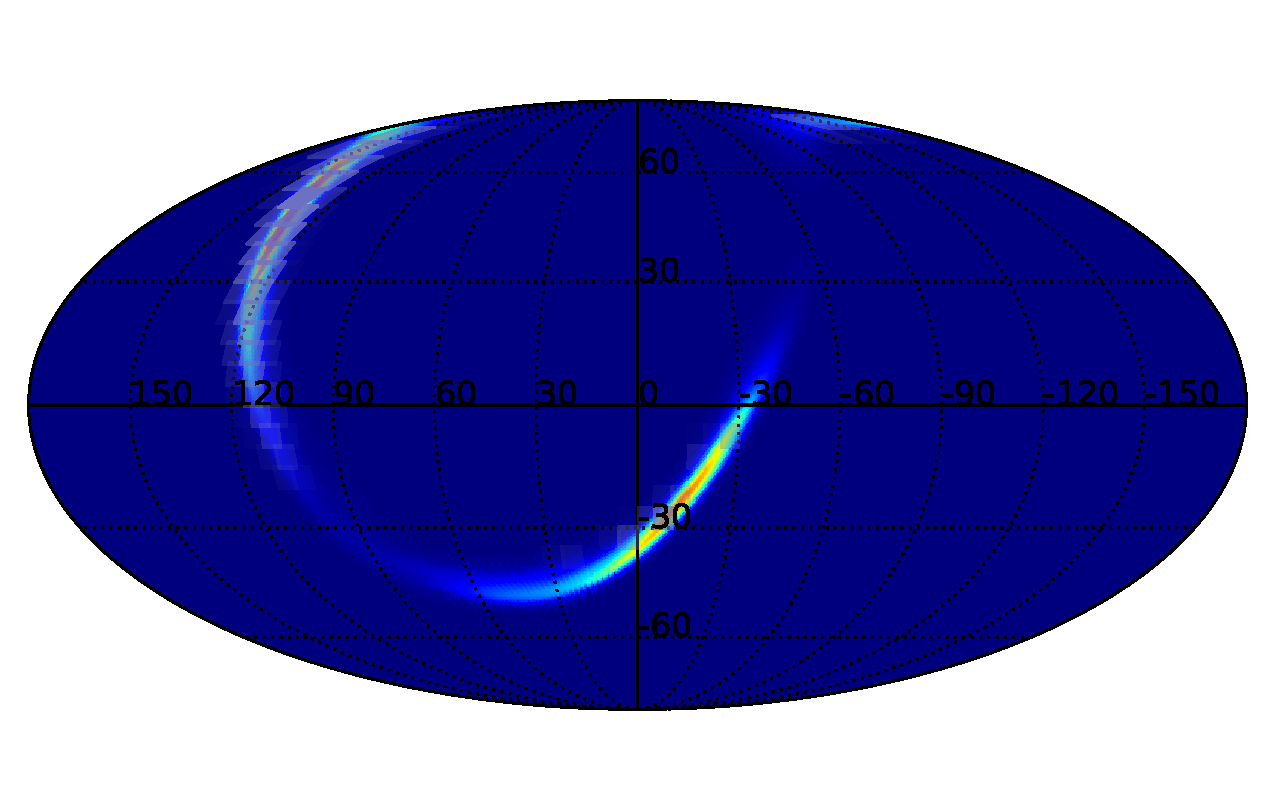
\includegraphics[width=3in]{timealloc_powerlaw}
    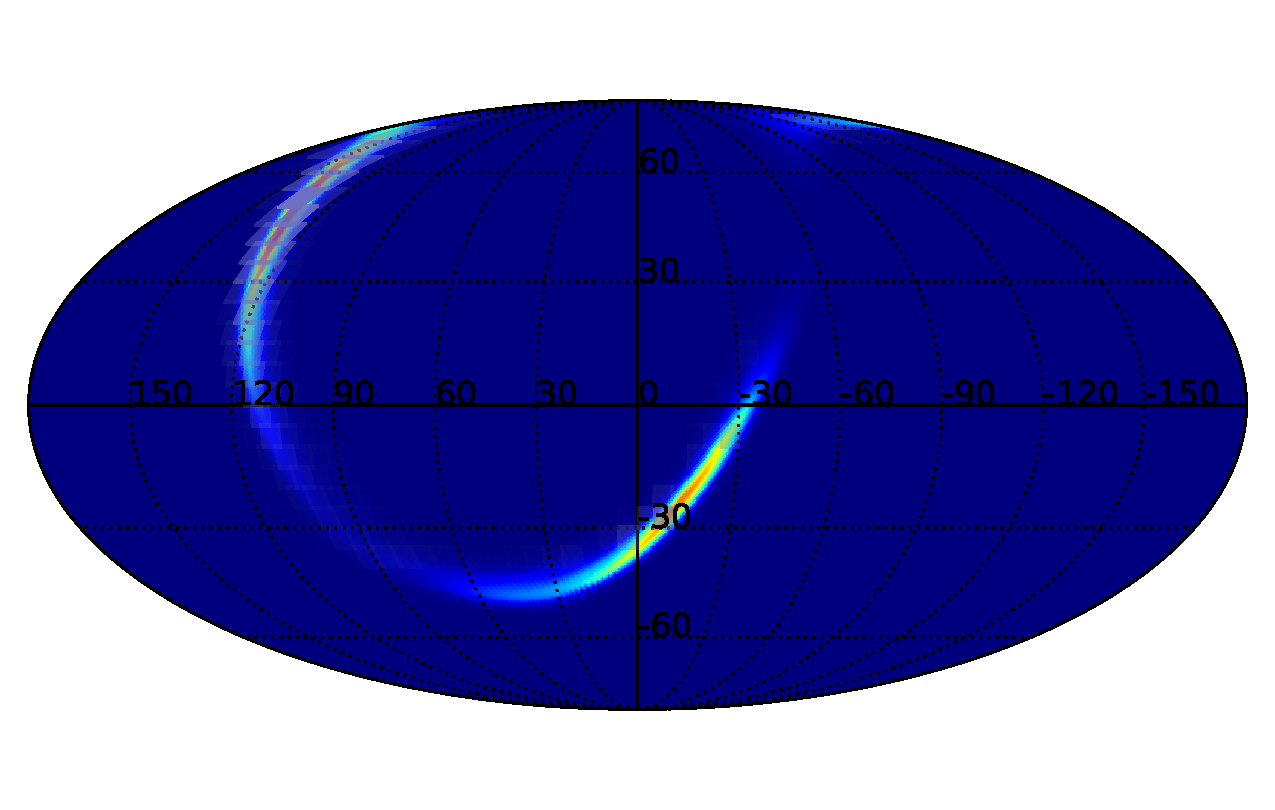
\includegraphics[width=3in]{timealloc_waw}
    \caption{Example outputs of different time allocation algorithms. On the top left is the tiles coverage with the PEM algorithm. On the top right is the tiles coverage with the Powerlaw algorithm. On the bottom is the tiles coverage with the WAW algorithm.}
    \label{fig:timealloc}
\end{figure*}


\subsection{Scheduling}
\begin{lstlisting}
python gwemopt_run --doEvent --doPlots --doTiles --doSchedule --scheduleType sear
\end{lstlisting}
Once the time allocated to each tile has been set, the next task is to schedule the observations that both best represent the time requested and optimize the times that are chosen in some way, for example, such that tiles are re-imaged at an approximately fixed cadence so as to measure possible lightcurve evolution or to go as deep as possible in one set.
Other optimizations might employ ordering based on airmass, as sources imaged through higher airmass will have lower signal-to-noise ratios due to scattering.

The time that each tile is available for observation above the altitude limit is computed.
Using the set of segments available to the telescope, these tile-specific segments  are intersected with these segments to form a set of visibility segments for each tile.
This has the benefit of avoiding issues related to simply tracking the rise and set times of each tile.

To account for lunar sky brightness, we use a model from \cite{CoSt2016b}. 
Any tile whose sky brightness is increased by at least 1\,mag is excluded.

There are three options related to scheduling observations, greedy, sear, and weighted.

\emph{Greedy.} The simplest version of scheduling employs a schedule simply on the basis of probability contained. The idea is that higher ranked tiles are observed before lower ranked tiles based on this ranking scheme. \cite{RaSi2017} implemented a greedy algorithm whereby the field with the highest probability region in a given time window is observed. As this analysis did not include the possibility of multiple exposures for each pointing, it is modified in the analysis to include multiple exposures. The algorithm is as follows:

\begin{enumerate}
\item Construct a list of the tiles and number of exposures for each tile based on the time allocation algorithm utilized.
\item For each window, find the sky tiles that are in the current window: $T_0 + (j-1) T_{exp}$ and $T_0 + j T_{exp}$
\item Allocate the window to the sky tile with the greatest probability, and increment the number of exposures for that tile down by 1.
\end{enumerate}

\emph{sear (Setting Array).} The greedy algorithm has the short-coming that it does not account for site visibility. This motivates re-ordering the sequence such that as many tiles can be imaged as possible.
\cite{RaSi2017} also implemented a version whereby the rising and setting of tiles were accounted for. It uses the idea that observes high probability tiles first, subject to the condition that each tile from the
observing sequence must be observed before it sets.

\emph{weighted.} Given the impossibility of necessarily observing all of the tiles as they rise and set given the requirement of using multiple exposures per tile, we are motivated to define a scheme whereby each tile is given a weight based on both gravitational-wave likelihood enclosed, the number of exposures required for that tile, and the number of available slots for it to be image. Therefore we define the weights $w_i$ as

\begin{equation}
w_i = L_\textrm{GW}(\alpha_i,\delta_i) \times \frac{N_\textrm{R}}{N_\textrm{A}} 
\end{equation}

\subsection{Efficiency}
\begin{lstlisting}
python gwemopt_run --doEvent --doPlots --doTiles --doSchedule --doEfficiency
\end{lstlisting}
We are able to test and compare the performance of these algorithms by performing simulated observations. 
We adopt observational constraints as follows. 
We use an observing limit of an altitude of 30$^\circ$, corresponding to an airmass of 2.0. 
We assume observations are available to begin at twilight and dawn, corresponding to when the sun is 12$^\circ$ below the western and eastern horizons.
We do not point away from the moon or account for sky brightness.

To estimate the efficiency for the ``detection'' of the electromagnetic counterparts to gravitational-wave transients, we perform simulated injections of supplied lightcurves. We provide example lightcurves for a variety of lightcurve models, including:

\begin{enumerate}
\item \cite{TaHo2014}: Simulations of binary systems showing ejecta morphology and resulting lightcurves.
These simulations led to analytical models for black-hole neutron star systems from \item \cite{KaKy2016}: Analytical models for black-hole neutron star systems based on \cite{TaHo2014}
\item \cite{DiUj2017}: Analytical models for binary neutron star systems based on \cite{TaHo2014}
\item \cite{BaKa2016}: Simulations of binary systems studying the emission profiles of radioactive decay products from the merger.
\item \cite{MeBa2015}: Blue ``precursor'' to the kilonovae driven by $\beta$-decay of the ejecta mass.
\end{enumerate}

The requirements for ``detection'' of the electromagnetic counterparts to gravitational-wave transients are as follows.
We require that the transient appear in \rednote{?} images over \rednote{?} nights.
In each image, the transient must exceed the limiting magnitude in that image.
The color of the transient is estimated from the filter given in the configuration file.
We simulate the transients at a variety of location and distances consistent with the gravitational-wave probability skymap.


\section{Performance}
\label{sec:performance}

\section{Conclusion}
\label{sec:conclusions}

\section{Acknowledgments}
MC is supported by National Science Foundation Graduate Research Fellowship Program, under NSF grant number DGE 1144152.

\bibliographystyle{aasjournal}
\bibliography{references}

\end{document} 
